\documentclass{sig-alternate-05-2015}
\usepackage{graphicx}
\usepackage{caption}
\usepackage{subcaption}


\newenvironment{myitemize}{\begin{itemize} \setlength{\topsep}{0pt} \setlength{\itemsep}{0pt} \setlength{\parskip}{0pt} \setlength{\parsep}{0pt}}{  \end{itemize} }

\setlength{\itemsep}{0pt}

\begin{document}

% Copyright
\CopyrightYear{2016} 
\setcopyright{rightsretained} 
\conferenceinfo{RecSys '16}{September 15-19, 2016, Boston , MA, USA} 
\isbn{978-1-4503-4035-9/16/09}
\doi{http://dx.doi.org/10.1145/2959100.2959207}

\clubpenalty=10000 
\widowpenalty = 10000


\title{RecSys Challenge 2016: Job Recommendations}

% Authors (in alphabetical order):
\numberofauthors{5} 

\author{
\alignauthor
Fabian Abel\\
       \affaddr{XING AG}\\
       \affaddr{Hamburg, Germany}\\
       \affaddr{fabian.abel@xing.com}
\alignauthor
Andr�s Bencz�r\\
       \affaddr{Hungarian Academy of Sciences}\\
       \affaddr{Budapest, Hungary}\\
       \affaddr{benczur@sztaki.hu}
\and
Daniel Kohlsdorf\\
       \affaddr{XING AG}\\
       \affaddr{Hamburg, Germany}\\
       \affaddr{daniel.kohlsdorf@xing.com}
\alignauthor 
Martha Larson\\
       \affaddr{TU Delft}\\
       \affaddr{Radboud University Nijmegen}\\
              \affaddr{Netherlands}\\
       \affaddr{m.a.larson@tudelft.nl}
\alignauthor 
R�bert P�lovics\\
       \affaddr{Hungarian Academy of Sciences}\\
       \affaddr{Budapest, Hungary}\\
       \affaddr{palovics@sztaki.hu}
}

\maketitle
\begin{abstract}
The 2016 ACM Recommender Systems Challenge focused on the problem of job recommendations.
Given a large dataset from XING that consisted of anonymized user profiles, job postings, and interactions between them, the participating teams had to predict postings that a user will interact with. 

The challenge ran for four months with 366 registered teams.
119 of those teams actively participated and submitted together 
4,232 solutions yielding in an impressive neck-and-neck race 
that was decided within the last days of the challenge.
\end{abstract}


%
% The code below should be generated by the tool at
% http://dl.acm.org/ccs.cfm
% Please copy and paste the code instead of the example below. 
%
{\small
\begin{CCSXML}
<ccs2012>
<concept>
<concept_id>10002951.10003317.10003347.10003350</concept_id>
<concept_desc>Information systems~Recommender systems</concept_desc>
<concept_significance>500</concept_significance>
</concept>
<concept>
<concept_id>10002951.10003227.10003351</concept_id>
<concept_desc>Information systems~Data mining</concept_desc>
<concept_significance>300</concept_significance>
</concept>
<concept>
<concept_id>10002951.10003317.10003359.10003360</concept_id>
<concept_desc>Information systems~Test collections</concept_desc>
<concept_significance>300</concept_significance>
</concept>
</ccs2012>
\end{CCSXML}

\ccsdesc[500]{Information systems~Recommender systems}
\ccsdesc[300]{Information systems~Data mining}
\ccsdesc[300]{Information systems~Test collections}


%
% End generated code
%

%
%  Use this command to print the description
%
\printccsdesc

% We no longer use \terms command
%\terms{Theory}

\keywords{Recommender Systems; Data Mining Challenge; XING}
}

\section{Introduction}
The ACM RecSys Challenge allows researchers and engineers around the world to jointly work on real-world recommender system problems in various domains such as social media~\cite{recsyschallenge:2014} or product recommendations~\cite{recsyschallenge:2015}. 
In 2016 the challenge was dedicated to the problem of job recommendation\footnote{\url{http://2016.recsyschallenge.com}}~\cite{job:recommendations}. 
We released a dataset from XING\footnote{\url{http://xing.com}}---a business-oriented social network with around 18~Million users world-wide and more than 10~Million users in Germany. 

XING supports people in discovering career opportunities. Job recommendations are therefore an essential part of the XING platform and its mobile apps.
Those recommendations aim to satisfy the demands of both the job seekers who have certain preferences concerning their next career step and the recruiters who aim to hire the most appropriate candidate for a given job.
In this challenge, we focused on the demands of the job seekers by defining the following task:
{\em Given a XING user, the recommender had to predict those job postings that a user will positively interact with by clicking on it or bookmarking it.}

  
\section{Dataset}
\begin{figure}
\centering
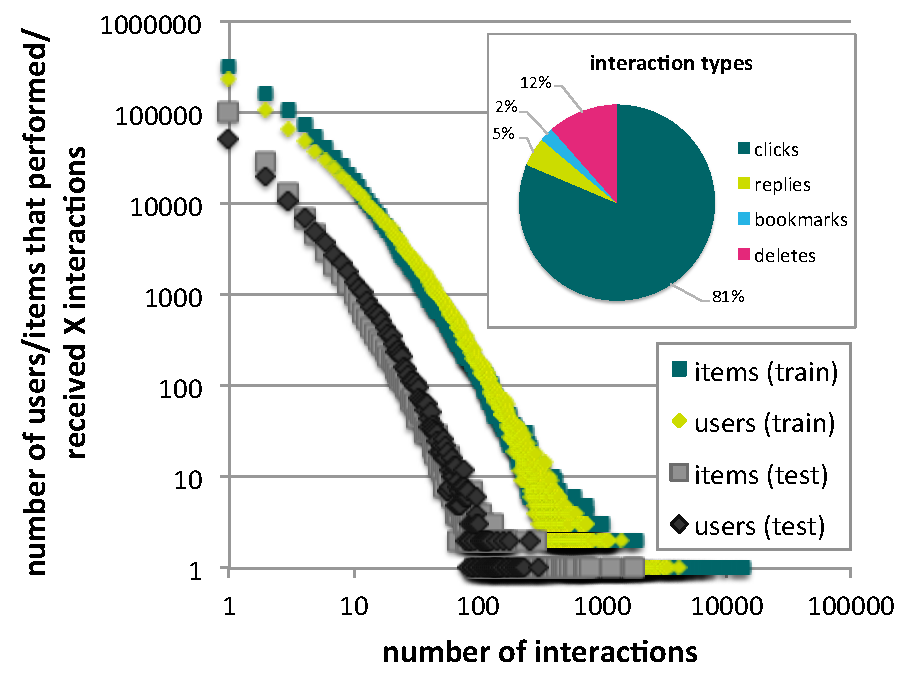
\includegraphics[width=0.45\textwidth]{data-interactions-combined.pdf}
\vspace{-0.3cm}
\caption{Number of interactions per user and item. 328,618 items (24.2\%) and 582,370 users (42.9\%) remained without interactions during the training period. More than 80\% of the interactions are clicks, followed by deletes, replies and bookmarks. The distributions for training data and test data (ground truth) follow similar characteristics.}
\label{fig:data-interactions}
\end{figure}

\begin{figure*}[t]
    \centering
    \begin{subfigure}[t]{0.3\textwidth}
        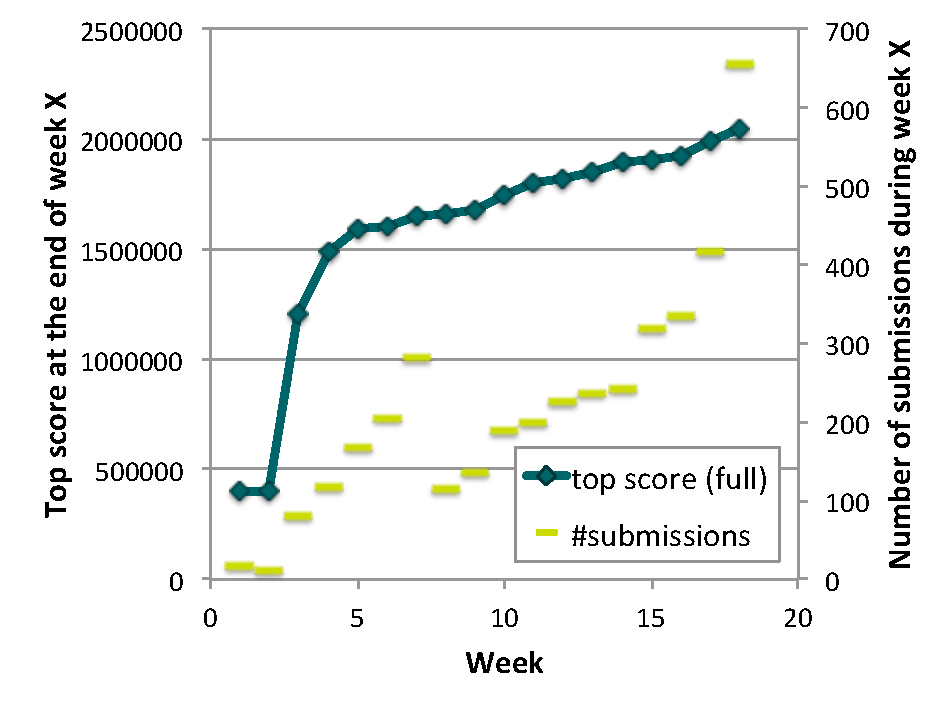
\includegraphics[width=\textwidth]{results-top-score-over-time.pdf}
  \caption{Top score over time and number of submissions during each week of the challenge.}
  \label{fig:results-scores-over-time}
    \end{subfigure}
    ~ %add desired spacing between images, e. g. ~, \quad, \qquad, \hfill etc. 
      %(or a blank line to force the subfigure onto a new line)
    \begin{subfigure}[t]{0.3\textwidth}
  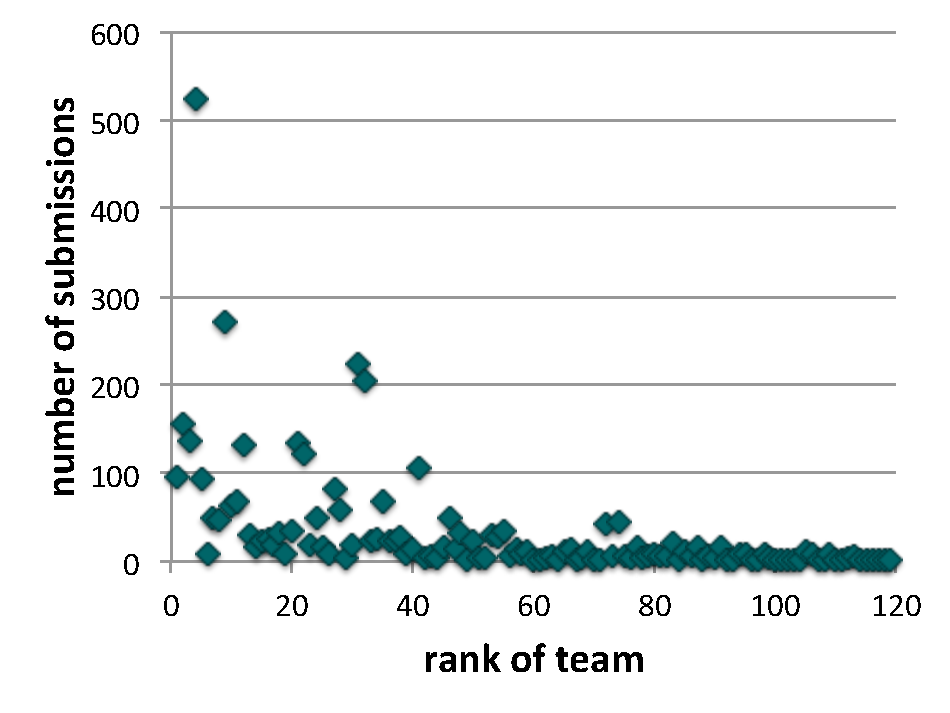
\includegraphics[width=\textwidth]{results-submissions-by-rank.pdf}
  \caption{Number of submissions per team (ordered by final rank of the team).}
  \label{fig:results-submissions-by-rank}
    \end{subfigure}
    ~ %add desired spacing between images, e. g. ~, \quad, \qquad, \hfill etc. 
    %(or a blank line to force the subfigure onto a new line)
    \begin{subfigure}[t]{0.3\textwidth}
  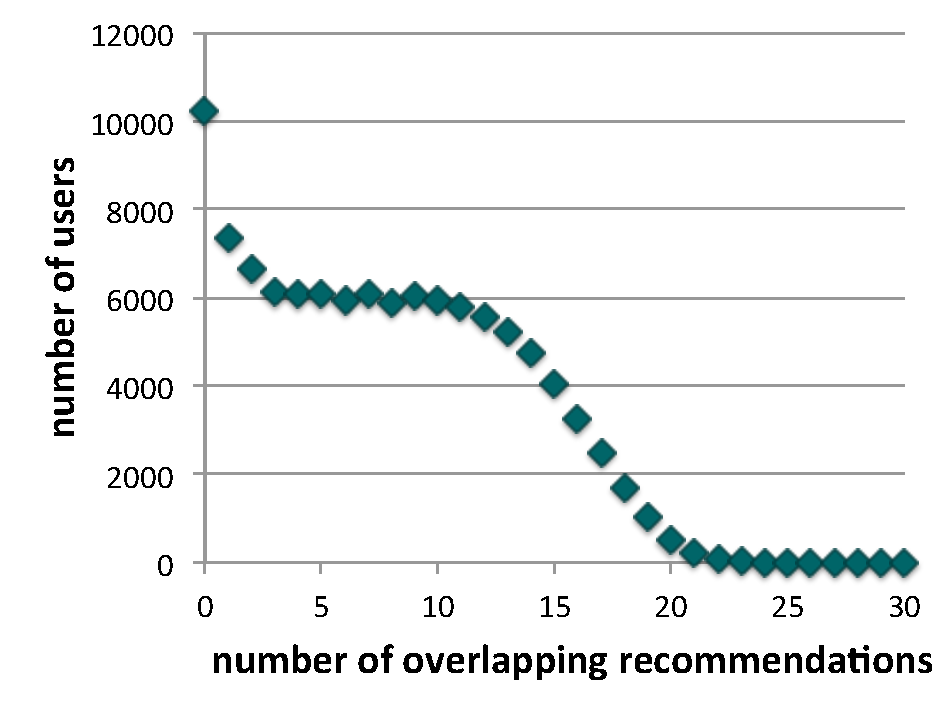
\includegraphics[width=\textwidth]{results-overlap-with-xing-recos.pdf}
  \caption{Overlap between top solution and recommendations generated by XING's job recommender.}
  \label{fig:results-overlap-xing}
    \end{subfigure}
    \caption{Submission statistics.}\label{fig:results}
\end{figure*}

We provided a training dataset featuring user profiles, job postings, and interactions that users performed on job posts.
The dataset also incorporated user-item \emph{impressions}, i.e.~information about job postings that were shown to users.
The training data\footnote{\url{https://github.com/recsyschallenge/2016/#data}} contained 1,367,057 users and 1,358,098 items. 
Users and items were described by several similar attributes such as job categories, career level, industry, location, etc.
In addition, the educational background and details about work experience were given for the users. 

Around 12 weeks of interaction data between the users and the items was released for training including 
including (1) \emph{clicks} on job postings, (2) \emph{bookmarks}, (3) \emph{replies} indicating that users intended to 
apply for the job and (4) \emph{deletes} which corresponds to removing an item that the user no longer wants to see.
Figure~\ref{fig:data-interactions} describes the characteristics of the different interactions.
Two weeks of interactions for a set of 150,000 \emph{target users} were used as test data in order to evaluate the submitted solutions. 
Figure~\ref{fig:data-interactions} also shows the distribution of that ground truth dataset. 


\subsection{Anonymization}
Anonymization of the training dataset was carried out with an iterative protector/attacker procedure. 
We took a simple and straightforward approach to threat modeling: 
The attacker profile was implicit the choice of a highly experienced Data Science team that 
attempted to de-anonymize the data. At each step the dataset was further bleached, and additional 
synthetic users were added. Then, tests were carried out to check if the dataset could be 
de-anonymized by the attacker and also if the dataset supported training a recommender system 
algorithm effective on a plain-text test set. This procedure ensured that enough information was 
left in the data to make this to be a useful data set for solving the problem on the actual 
plain-text data, while at the same time protecting the privacy of XING users. 

The bleaching procedure involved replacing named entities with IDs, removing a selection of 
user attribute values, and removing a selection of interactions. The relative ordering of the 
interactions was maintained. Synthetic users were created by clustering real users. Further 
protections included the obvious measure of including only a fraction of XING's users and job 
postings in the dataset, and also protecting the dataset legally with a user agreement that 
explicitly prohibits attempts to de-anonymize the dataset, share it, or use it for 
non-academic purposes.

\section{Challenge Setup and Results}

We used a scoring function as evaluation measure that combines precision@k and recall@k\footnote{\url{https://github.com/recsyschallenge/2016/#evaluation}}. 
This evaluation measure was based on the key performance indicators that XING is using to monitor the quality of the job recommender system. 
Each team was allowed to submit 5~solutions per day and solution files were allowed to feature at most 30~recommendations per user.
A public leaderboard that was based on 30\% of the ground truth data immediately informed the teams about the performance of their algorithms after their submissions. 

The participating teams came from more than 30~different countries such as USA (25\%), Germany (11\%), China (9\%), France (7\%) or Hungary (4\%).
Teams came both from academia ($\sim$25\%) and industry ($\sim$75\%, most common: \textit{Internet \& IT}), e.g. from larger companies such as Yandex or Amazon as well as from smaller start-up companies. 

The evolution of the top full score---based on the entire ground truth---is depicted 
in Figure~\ref{fig:results-scores-over-time} together with the number of submissions that 
were performed during that week.
The top score thus increased from week to week.
In fact, the highest score of the challenge was achieved just 30~minutes before the official submission deadline.
Figure~\ref{fig:results-submissions-by-rank} reveals that not only the top teams very highly active in submitting solutions, but also many teams that finally ended up at rank 30 and above submitted a high number of solutions. 

The top solution achieved a score of 2,052,185 points that is 24.1\% of the best possible score.
Figure~\ref{fig:results-overlap-xing} also shows that the top solution managed to include items that XING's system does not recommended.
Hence, algorithms developed during the challenge seem to complement XING's recommender ensemble and are likely to have a significant impact on XING's future job recommendations. 

\paragraph*{Acknowledgments}
{\small
The work leading to these results has received funding from the EU's 
Seventh Framework Programme (FP7/2007-2013) under CrowdRec
Grant Agreement no.~610594.
}
% \bibliographystyle{abbrv}
% \bibliography{sigproc}  % sigproc.bib is the name of the Bibliography in this case
\begin{thebibliography}{3}

\bibitem{job:recommendations}
F.~Abel.
\newblock We know where you should work next summer: Job recommendations.
\newblock In {\em Proceedings of ACM RecSys 2015}, pages 230--230, 2015. ACM.

\bibitem{recsyschallenge:2015}
D.~Ben-Shimon, A.~Tsikinovsky, M.~Friedmann, B.~Shapira, L.~Rokach, and J.~Hoerle.
\newblock RecSys Challenge 2015 and the YOOCHOOSE Dataset.
\newblock In {\em Proceedings of ACM RecSys 2015}, pages 357--358, 2015. ACM.

\bibitem{recsyschallenge:2014}
A.~Said, S.~Dooms, B.~Loni, and D.~Tikk.
\newblock Recommender Systems Challenge 2014.
\newblock In {\em Proceedings of ACM RecSys 2014}, pages 387--388, 2014. ACM.

\end{thebibliography}

\end{document}
